% Revised manuscript draft[cite: 3]
\documentclass[conference]{IEEEtran}
\usepackage{amsmath,amssymb}
\usepackage{graphicx}
\usepackage{booktabs}
\usepackage{multirow}
\usepackage[hidelinks]{hyperref}
\usepackage{cite}
\usepackage{textcomp}

\begin{document}

\title{Does Explainability Survive Domain Shift?\\
A Quantitative Audit of Grad-CAM Faithfulness in PCOS Ultrasound Classification}

\author{
\IEEEauthorblockN{Mohammad Kawsar}
}

\maketitle

\begin{abstract}
Deep learning classifiers for polycystic ovary syndrome (PCOS) diagnosis from transvaginal ultrasound are commonly accompanied by post-hoc explanations such as Grad-CAM, which are typically validated only qualitatively, by visual inspection of a small number of heatmaps. This paper presents a quantitative audit of one such pipeline, combining a data-quality check with a faithfulness evaluation across three test conditions of increasing distributional distance from training data. We find that (1) the public PCOSGen dataset contains substantial internal near-duplication (32.2\% of training images share a near-identical counterpart) and cross-split contamination (17.4\% of the official test set duplicates a training image), but excluding these duplicates does not meaningfully change reported accuracy; (2) a naive random train/test split does not measurably inflate performance relative to a duplicate-aware split, despite 23.3\% of its test images having a near-duplicate in training; (3) Grad-CAM explanations are reliably more informative than a random-saliency baseline under an insertion-AUC metric across all three test conditions ($p < 2 \times 10^{-31}$ in every case), but are statistically indistinguishable from random under a deletion-AUC metric, an asymmetry that becomes complete ($p = 0.84$) on an independent external dataset; and (4) classification accuracy collapses to 31.1\% -- below the majority-class baseline -- on an external dataset whose class balance is inverted relative to training, despite an AUC of 0.72 that would suggest reasonable discriminative ability. These findings suggest that a single faithfulness metric, and a single in-distribution accuracy figure, are each insufficient to certify that an explainable clinical imaging model is trustworthy under real-world deployment conditions.
\end{abstract}

\begin{IEEEkeywords}
explainable AI, Grad-CAM, faithfulness evaluation, PCOS, ultrasound classification, dataset duplication, domain shift
\end{IEEEkeywords}

\section{Introduction}

Polycystic ovary syndrome (PCOS) is a common endocrine disorder, and its diagnosis is increasingly supported by convolutional neural network (CNN) classifiers applied to transvaginal ultrasound images. A substantial and growing body of work reports high classification accuracy on public PCOS ultrasound datasets, frequently paired with Grad-CAM or SHAP visualizations offered as evidence that the model attends to clinically relevant ovarian structures. In the majority of this literature, that evidence is qualitative: a handful of example heatmaps are shown and judged by eye to look anatomically plausible.

This pattern is not unique to PCOS. It reflects a broader tendency in applied medical-imaging machine learning to treat explainability as a box to check rather than a claim to test. Two specific gaps motivate the present study. First, near-duplicate images are a known issue in scraped or crowdsourced medical image datasets, and a duplicate that appears on both sides of a train/test split inflates reported performance in a way that is easy to overlook. Second, deletion and insertion AUC -- the standard quantitative faithfulness metrics in the explainability literature -- are rarely reported for PCOS classifiers, and are almost never compared against a random-saliency baseline of matched spatial structure, which is necessary to know whether an explanation method is doing better than chance.

This paper addresses both gaps for one representative pipeline: a transfer-learned ResNet18 classifier trained on the public PCOSGen dataset, evaluated with Grad-CAM. We make four contributions: (1) a perceptual-hash duplicate audit of PCOSGen, both within the training set and across its official train/test split; (2) a controlled comparison of a duplicate-aware (``group'') split against a naive random split, to directly measure whether leakage inflates reported accuracy; (3) a quantitative faithfulness evaluation using deletion and insertion AUC against a random-saliency baseline, replicated across three test conditions -- an in-distribution held-out split, the official same-source test set, and an independent external dataset; and (4) a calibration analysis showing how the model's performance degrades under a class-balance shift between training and deployment populations.

\section{Related Work}

Numerous studies have applied CNN or ensemble classifiers to public PCOS ultrasound datasets, reporting accuracies in the 84--97\% range, frequently with Grad-CAM visualizations offered as qualitative evidence of clinical plausibility; a 2026 systematic review catalogued a substantial number of these papers. Separately, a recent preprint auditing the PCOSGen dataset (introduced for the Auto-PCOS Classification Challenge) identified meaningful image duplication within it using perceptual hashing, though without connecting this to downstream model evaluation. The present work is, to our knowledge, the first to combine a duplicate audit with a quantitative, random-baseline-controlled faithfulness evaluation for this task, and the first to test whether either accuracy or explanation faithfulness for a PCOS classifier survives evaluation on an independent, differently-sourced dataset.

More broadly, the use of deletion/insertion curves to evaluate saliency-map faithfulness follows established practice in the explainability literature (e.g., the RISE framework of Petsiuk et al.), and the practice of comparing an explanation method against a random baseline of matched spatial structure is a standard sanity check that is nonetheless inconsistently applied in applied medical-imaging papers.

\section{Data}

\subsection{PCOSGen (primary dataset)}

PCOSGen is the dataset released for the Auto-PCOS Classification Challenge, comprising transvaginal ultrasound images gathered from public sources and annotated by gynaecologists. We use PCOSGen-train (3,200 images; Zenodo record 14592001) for model training, and the official PCOSGen-test set (1,468 images; Zenodo record 10510879) as a same-source held-out evaluation set. Each image carries two binary labels: whether the scan appears normal or abnormal, and whether polycystic ovarian morphology is visible. We use the normal/abnormal label as the classification target throughout. PCOSGen-train is class-imbalanced: 903 normal (28.2\%) and 2,297 abnormal (71.8\%) images. PCOSGen-test has a near-identical balance (416 normal, 28.3\%; 1,052 abnormal, 71.7\%).

\subsection{External dataset}

As an independent, differently-sourced test set, we use a publicly available Kaggle PCOS ultrasound dataset (``PCOS detection using ultrasound images''), organized into infected/notinfected class folders. We found that, for the infected class, all 781 filenames present in the smaller (train) folder also appear in the larger (test) folder, i.e.\ this dataset's own ``test'' split is not independent of its ``train'' split for that class; given the near-identical counts for the notinfected class (1,143 vs.\ 1,145), we assume, but did not directly verify, that the same holds there. We therefore use only the larger (test) folder (787 infected, 1,145 notinfected; 1,932 images total) as a single external evaluation set, and do not train on any part of it. Ten images (0.5\%) in this folder were zero-byte files -- several with WhatsApp-generated filenames, suggesting the dataset was partly assembled from informally shared images -- and were excluded automatically by our data loader. This external dataset's class balance (1,141 notinfected, 59.4\%; 781 infected, 40.6\%, after removing corrupt files) is the reverse of PCOSGen's: normal is the majority class here, whereas abnormal is the majority class in PCOSGen.

\section{Methods}

\subsection{Model and training}

We fine-tune a ResNet18 (ImageNet-pretrained) with a new binary classification head, using the Adam optimizer (learning rate $1\times10^{-4}$, batch size 32) for 15 epochs. Images are resized to $224\times224$ and normalized with standard ImageNet statistics; training images additionally receive random horizontal flips and $\pm10^{\circ}$ rotations. The checkpoint with the highest validation AUC is retained for evaluation.

\subsection{Duplicate detection}

We compute a perceptual hash (pHash) for every image and flag pairs with Hamming distance below a threshold as near-duplicates, using union-find to group transitively-linked images into clusters. We found that thresholds of 2 or more produced implausibly large clusters (the single largest reached 376 images at the default threshold, and 2,413 of 3,200 images, i.e.\ 75.4\%, belonged to some multi-image cluster at threshold 4) -- far more than a plausible number of repeat scans of one patient, consistent with unrelated ultrasound frames (which share a similar dark, fan-shaped acquisition geometry) chaining together transitively through the union-find grouping rather than being genuine duplicates. We did not visually inspect clusters at these looser thresholds and infer the chaining behavior from cluster-size implausibility alone. We therefore use threshold 0 (identical hash) throughout, which produces much smaller, more plausible clusters; we manually verified by visual inspection that the largest such cluster (33 images) contained genuine near-copies of the same underlying scan at different crops or scales, not unrelated images.

\subsection{Split strategy and leakage test}

To measure whether duplicate images inflate reported performance, we train the same model twice on PCOSGen-train: once with a group-aware split (GroupShuffleSplit) that constrains every image in a duplicate cluster to the same partition, and once with a naive random split of the same size ratios (70/15/15 train/validation/test). We report, for each split, the fraction of test (and validation) images that have a near-duplicate in the training partition, and compare final test-set accuracy and AUC between the two.

\subsection{Cross-dataset contamination check}

We additionally hash every image in PCOSGen-test and in the external Kaggle dataset and compare each against every image in PCOSGen-train, flagging cross-dataset near-duplicates at the same threshold. Where contamination is found, we report both the raw evaluation and a contamination-excluded evaluation on the same checkpoint.

\subsection{Faithfulness evaluation}

We generate Grad-CAM attribution maps from the final convolutional block of the trained ResNet18. Faithfulness is quantified via deletion and insertion AUC: for deletion, the most-important pixels (per Grad-CAM) are progressively replaced with a blurred version of the image ($11\times11$ average pooling) in 20 steps, and the model's predicted-class probability is tracked as a function of the fraction of pixels removed -- a faithful explanation should show a rapid probability drop, i.e.\ a low area under this curve. Insertion runs the same procedure in reverse, starting from the fully blurred image and progressively revealing the most-important pixels; a faithful explanation should show a rapid probability rise, i.e.\ a high area under this curve.

Critically, we compare Grad-CAM's deletion/insertion AUC against a random-saliency baseline generated at the same coarse spatial resolution as the Grad-CAM map (bilinearly upsampled from a $7\times7$ grid, matching ResNet18's final feature-map resolution, so that the comparison isolates which pixels are chosen rather than how spatially coherent the chosen region is), averaged over three random draws per image. We evaluate on a random sample of 200 images per test condition and assess statistical significance with a paired Wilcoxon signed-rank test comparing Grad-CAM's AUC against the matched random-saliency AUC across the 200 image pairs.

\section{Results}

\subsection{Duplicate audit}

At hash threshold 0, 1,030 of 3,200 PCOSGen-train images (32.2\%) belong to a near-duplicate cluster of size $\geq 2$ (390 such clusters; the three largest contain 33, 27, and 13 images respectively; 160 images are byte-identical to another image in the set). Manual inspection of the largest cluster confirmed these were the same underlying scan saved at different crops and zoom levels (pixel-level difference of 4--16 on a 0--255 scale after downsampling to $64\times64$), not merely visually similar unrelated scans; byte-identical duplicates within the same dataset (160 images) trivially have zero difference by construction.

\subsection{Leakage inflation test}

\begin{table}[t]
\centering
\caption{Group-aware vs.\ random train/test split}
\label{tab:leakage}
\begin{tabular}{@{}lcccc@{}}
\toprule
Split & Test dup.\ in train & Acc. & F1 & AUC \\
\midrule
Group-aware (clean) & 0.0\% & 0.759 & 0.844 & 0.839 \\
Random (naive) & 23.3\% & 0.769 & 0.857 & 0.813 \\
\bottomrule
\end{tabular}
\end{table}

Despite 23.3\% of the random split's test set having a near-duplicate in the training partition, test AUC under the random split (0.813) was not higher than under the group-aware split (0.839); accuracy was marginally higher under the random split (0.769 vs.\ 0.759), but the random split's test set is also more skewed toward the majority class (73.8\% vs.\ 67.4\% abnormal), which alone would raise a majority-baseline accuracy by 6.4 points. We conclude that, for this model and this degree of contamination, duplicate leakage between a random train/test split did not produce a detectable performance inflation -- plausibly because the model does not memorize individual training images (training accuracy plateaus near 81\% with data augmentation, well short of the near-100\% that would indicate memorization).

\subsection{Cross-dataset contamination}

255 of 1,468 PCOSGen-test images (17.4\%) have a near-duplicate in PCOSGen-train, indicating that the official PCOSGen train/test split is itself not fully independent. 95 of 1,922 external Kaggle images (4.9\%) also have a near-duplicate in PCOSGen-train, suggesting partial overlap in underlying image sources between the two datasets. In both cases, excluding the contaminated images changed accuracy by at most about 1.7 percentage points (1.71 for PCOSGen-test, 0.13 for the external set), in the direction opposite to what leakage-driven inflation would predict (Section~V-B), indicating that contamination is not the primary driver of the accuracy patterns reported below.

\subsection{Classification performance across test conditions}

\begin{table*}[t]
\centering
\caption{Classification performance across test conditions}
\label{tab:classification}
\begin{tabular}{@{}lccccc@{}}
\toprule
Test condition & $n$ & Accuracy & F1 & AUC & Majority-class baseline \\
\midrule
In-distribution held-out & 478 & 0.759 & 0.844 & 0.839 & 0.674 \\
PCOSGen-test (contamination-excluded) & 1,213 & 0.879 & 0.920 & 0.962 & 0.714 \\
External Kaggle (contamination-excluded) & 1,827 & 0.311 & 0.473 & 0.720 & 0.588 \\
\bottomrule
\end{tabular}
\end{table*}

The model performs best on PCOSGen-test, moderately on its own held-out split, and far below chance-adjusted expectation on the external dataset -- 31.1\% accuracy against a 58.8\% majority-baseline (always predicting ``notinfected''). Despite this, AUC on the external set (0.720) remains well above 0.5, indicating the model retains meaningful discriminative signal; the failure is one of decision threshold, not of learned representation. We attribute this to the model's strong bias toward predicting ``abnormal'' (86.5\% of in-distribution predictions, 77.0\% of PCOSGen-test predictions, 87.5\% of external predictions), learned from PCOSGen-train's 71.8\% abnormal prevalence, colliding with the (contamination-excluded) external evaluation set's inverted 41.2\% abnormal prevalence.

\subsection{Faithfulness results}

\begin{table*}[t]
\centering
\caption{Deletion and insertion AUC: Grad-CAM vs.\ random saliency}
\label{tab:faithfulness}
\begin{tabular}{@{}lcccccc@{}}
\toprule
Condition & Del.\ Grad-CAM & Del.\ random & Del.\ $p$ & Ins.\ Grad-CAM & Ins.\ random & Ins.\ $p$ \\
\midrule
In-distribution held-out & 0.648 & 0.643 & 0.042 & 0.742 & 0.639 & $1.1\times10^{-32}$ \\
PCOSGen-test (clean) & 0.773 & 0.782 & 0.057 & 0.885 & 0.778 & $5.8\times10^{-34}$ \\
External Kaggle (clean) & 0.685 & 0.686 & 0.84 & 0.816 & 0.683 & $2.6\times10^{-34}$ \\
\bottomrule
\end{tabular}
\end{table*}

\begin{figure*}[t]
\centering
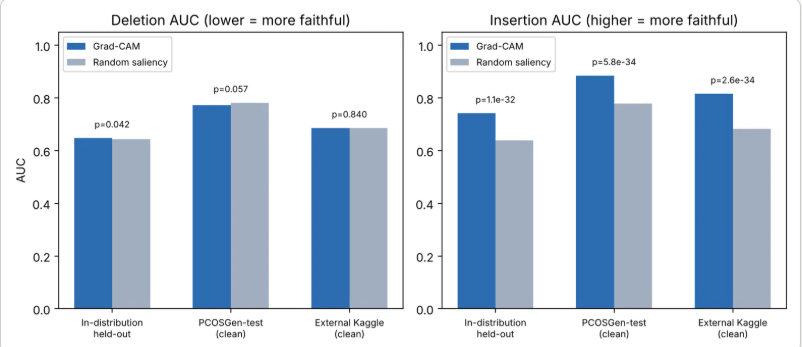
\includegraphics[width=0.85\textwidth]{faithfulness_comparison.png}
\caption{Grad-CAM vs.\ random-saliency deletion and insertion AUC across three test conditions. Error is not shown (single-seed evaluation; see Limitations).}
\label{fig:faithfulness}
\end{figure*}

Fig.~\ref{fig:faithfulness} visualizes this pattern. Insertion-AUC faithfulness is large and highly statistically significant in every test condition ($p$ ranging from $2.6\times10^{-34}$ to $1.1\times10^{-32}$): the regions Grad-CAM identifies as important are consistently more informative than random regions of matched spatial structure. Deletion-AUC faithfulness tells a different story: the gap between Grad-CAM and random narrows as test conditions move further from the training distribution, and on the external dataset it disappears entirely (0.685 vs.\ 0.686, $p = 0.84$) -- masking Grad-CAM's top-ranked pixels is no more damaging to the model's prediction than masking an equivalent random region.

We note a plausible mechanism for this asymmetry: mean model confidence on the fully blurred (maximally uninformative) image remains high across all conditions -- 0.709 in-distribution, 0.793 on PCOSGen-test, 0.700 on the external set -- compared to confidence on the original image (0.822, 0.960, 0.915 respectively). Because deletion AUC is bounded below by this residual confidence, a model that stays confident even with almost no visual information available has limited room for any explanation method, faithful or not, to demonstrate a further probability drop. This residual-confidence ceiling, itself a symptom of the calibration issue described in Section~V-D, may be suppressing the deletion metric's ability to discriminate Grad-CAM from random baseline, independent of whether Grad-CAM's spatial attributions are themselves informative -- which the insertion metric suggests they are.

\section{Discussion}

Three findings are relevant to how explainability claims for medical imaging classifiers should be evaluated and reported.

First, near-duplicate contamination that would concern a careful reviewer (32.2\% within-set duplication, 17.4\% train/test contamination in a widely-used public dataset) did not, in this case, translate into a measurable accuracy inflation. This is a useful negative result: it suggests that duplicate contamination and leakage-driven score inflation are separate phenomena that must each be tested for directly, rather than one being assumed to imply the other. A dataset can be contaminated without its evaluation being fooled by that contamination, provided the trained model does not memorize individual images.

Second, and most centrally, Grad-CAM's two standard faithfulness metrics diverge under domain shift. Insertion faithfulness is robust: it holds up, with overwhelming statistical significance, even on a completely independent, differently-sourced dataset. Deletion faithfulness is fragile: already only marginally significant in-distribution ($p = 0.042$), it is statistically indistinguishable from random by the time the model is evaluated on external data. A practitioner who validated this model's explanations using only one of these two standard metrics would reach opposite conclusions about whether Grad-CAM is trustworthy -- which argues against relying on either metric alone, and specifically against relying on deletion AUC as evaluated in-distribution as a general-purpose faithfulness certificate, since it may not reflect faithfulness under the conditions the model will actually encounter in deployment.

Third, the collapse in raw accuracy on the external dataset (31.1\%, well below even the majority-class baseline of 58.8\%) despite a retained, respectable AUC (0.720) illustrates a distinct and clinically important failure mode: a model can preserve its ability to rank patients correctly by risk while making systematically wrong hard decisions, if its decision threshold was implicitly tuned to a training population's class balance that does not match the deployment population. This is a calibration problem, not a representation-learning problem: neither an accuracy figure computed only in-distribution, nor an AUC value alone, would reveal it, since AUC is insensitive to decision-threshold miscalibration and in-distribution accuracy does not expose how that threshold performs under a different class balance.

\section{Limitations}

\begin{itemize}
\item All results derive from a single training run (one random seed) per split configuration; the leakage-inflation comparison in particular (Section~V-B) rests on a gap (0.813 vs.\ 0.839 AUC) that is plausibly within single-seed noise, and should be treated as suggestive rather than conclusive without multi-seed replication.
\item A single architecture (ResNet18) and a single explanation method (Grad-CAM) were evaluated; findings may not generalize to other architectures or to other explanation methods (e.g.\ SHAP, LIME, or attention-based explanations).
\item Faithfulness metrics were computed on a random sample of 200 images per test condition rather than the full test set, for computational tractability; this does not affect the validity of the paired statistical tests but does mean the point estimates carry sampling variance not reflected in the $p$-values, which concern only Grad-CAM vs.\ random within the sampled set.
\item The deletion/insertion procedure uses a blur baseline; results were not cross-checked against a black-image or mean-pixel baseline, which prior work has shown can affect deletion/insertion AUC values.
\item Duplicate detection used a single perceptual-hash threshold (identical hash only); a small number of near-duplicates with minor edits (e.g.\ cropping beyond what preserves an identical hash) may remain undetected, meaning the reported duplication rates are a lower bound.
\item Training was conducted without correcting for PCOSGen-train's class imbalance (e.g.\ no class weighting or resampling); the calibration failure reported in Section~V-D is consistent with, though not proven to be caused solely by, this choice.
\item Model training and evaluation was conducted on CPU hardware; this does not affect result validity but limited the number of training runs feasible within the scope of this study.
\end{itemize}

\section{Conclusion}

We presented a quantitative audit of a representative PCOS-ultrasound explainable-AI pipeline, testing claims that are typically asserted qualitatively or left untested in this literature. We found that duplicate contamination, while substantial, did not measurably inflate reported performance in this instance; that Grad-CAM's two standard faithfulness metrics disagree with each other, with deletion faithfulness specifically failing to survive evaluation on independent data; and that a respectable AUC can coexist with catastrophic accuracy under a plausible, realistic deployment shift in class balance. We recommend that future work reporting explainability for clinical imaging models report both deletion and insertion faithfulness against an explicit random-saliency baseline, evaluate on at least one dataset independent of the training source, and report calibration-sensitive metrics (not AUC alone) under a class-balance shift representative of intended deployment settings.

\*{Data and Code Availability}

PCOSGen-train and PCOSGen-test are available from Zenodo (records 14592001 and 10510879 respectively) under the Auto-PCOS Classification Challenge. The external evaluation dataset is publicly available on Kaggle. All training, evaluation, and duplicate-detection code used in this study is available at [repository URL to be inserted by author].

\begin{thebibliography}{9}

\bibitem{ref1}
[Author(s)], ``A systematic review of deep learning approaches for PCOS classification from ultrasound imaging,''